%!TEX root = ../main.tex

\chapter{Project Draft}
\label{ch:project_draft}

\section{Goals}\label{sec:goals}
The overall goal of the project is to develop a GIS-based system for managing and providing public access to the master plan data for the municipality of Fano.

\subsection{Detailed Goals:}\label{subsec:detailed-goals:}
\begin{enumerate}
    \item Create an interactive web map application that allows citizens to view the current master plan and look up zoning information for specific parcels
    \item Develop an editing plugin for municipal technicians to create, edit, and manage master plan variants
    \item Integrate parcel/cadastral data to support parcel ID lookups and displaying zoning on individual parcels
    \item Implement a central PostGIS database for master plan data and integrate with existing municipal IT infrastructure
    \item Follow best practices for web mapping architecture, data standards, and security
\end{enumerate}

\subsection{Intermediate Goals:}\label{subsec:intermediate-goals:}
\begin{enumerate}
    \item Complete market analysis and requirements gathering
    \item Design system architecture and draft plan for integration with municipal IT environment
    \item Develop prototype web map application for public zoning lookups
    \item Develop prototype OpenJUMP plugin for master plan variant editing
    \item Integrate sample datasets and test parcel lookup and zoning identification functionality
    \item Deliver prototypes to the customer for approval
    \item Develop full web map application and OpenJUMP plugin based on prototypes
    \item Deploy integrated system to municipal infrastructure
    \item Load final master plan dataset into PostGIS database
    \item Train municipal technicians on using OpenJUMP plugin
    \item Promote web map application access to public
\end{enumerate}


The intermediate goals aim to break the project into manageable milestones, deliver incremental prototypes for feedback, and ensure the final system meets the requirements identified early in the process. The prototypes provide an opportunity for validating functionality and usability before committing to full system development.


\section{Technological Components}\label{sec:technological-components}
The technological components of our GIS project are instrumental in realizing the vision of an efficient and user-friendly Master Plan management application. These components encompass both software and hardware aspects, with careful consideration given to the tools that facilitate seamless interaction, data management, and system performance.

\subsection{Database}\label{subsec:database}
The system's database serves as the central component connecting all other technological elements.
Moreover, the customer's existing IT department already possesses a PostgreSQL database, which seamlessly aligns with our development needs.
This is thanks to its PostGIS extension, designed for handling spatial and geographical data, making it an ideal foundation for our application's development.

\subsection{Desktop GIS System (Plugin)}\label{subsec:openjump-plugin}
In accordance with specified criteria, the OpenJUMP plugin operates and helps by loading plan and variant layers, visualizing affected cadastral particles, identifying misaligned boundaries, and showcasing excluded or partially included parcels.
Moreover, it accurately measures gaps between variant and cadastral parcel edges, highlighting sections within a 1-meter threshold in a new layer.
This systematic process efficiently addresses functional requirements, facilitating precise geospatial analysis.

\subsection{WebGIS Application}\label{subsec:webgis-application}
The central component of the system will be the web application, which must offer GIS capabilities and integrate various components:

\begin{table}[htbp]
    \centering
    \renewcommand{\arraystretch}{1.1}
    \begin{tabular}{|l|p{9cm}|}
        \hline
        \textbf{Component} & \textbf{Description} \\
        \hline
        \textbf{Frontend Map Management} & Integration of the Leaflet JavaScript plugin to allow users to utilize maps within the web app. \\
        \hline
        \textbf{Background Map} & Displaying a province-level background map using OpenStreetMap maps within the Leaflet library. \\
        \hline
        \textbf{Backend Spatial Data Delivery} & Utilizing a dedicated Geoserver instance to deliver and display the spatial data available from the Pesaro-Urbino Region. \\
        \hline
        \textbf{Frontend Implementation} & Ensuring certain parts of the web application are accessible to provincial citizens on mobile devices. Implementing full responsiveness to make the system usable on any terminal, including smartphones and tablets. The Bootstrap Italia template is chosen for better integration with other public IT systems. \\
        \hline
    \end{tabular}
    \caption{WebGIS Application central components \label{tab:table-web-components}}
\end{table}

\newpage

\subsection{Software Requirements}\label{subsec:software-requirements}
Many softwares needs to be used to set up the system:
\begin{enumerate}
    \item \textbf{Database}, utilize PostgreSQL 15 as the relational database management system (RDBMS), chosen for its stability, performance, and support for geospatial data manipulation. Additionally, the system shall incorporate the PostGIS extension 2.5.2 into the PostgreSQL database.

    \item \textbf{Docker}, is a platform that allows you to develop, deploy, and run applications in isolated containers. Containers are lightweight, portable, and self-sufficient units that encapsulate an application along with its dependencies, enabling consistent and efficient deployment across different environments.
    
    \item \textbf{Web Map Service (WMS)}, a system capable of delivering web maps is needed: for this, Geoserver is the best solution available.
    
    \item \textbf{Tools, Frameworks \& Libraries:}
    \begin{enumerate}
        \item \textbf{FastAPI:} FastAPI is a modern, fast (high-performance), web framework for building APIs with Python 3.6+ based on standard Python type hints.

        \item \textbf{caddy-server:} Caddy 2 is a powerful, enterprise-ready, open source web server with automatic HTTPS written in Go and used as a reverse proxy, which uses namespaces routing,
        
        \item \textbf{Minio server:} This template allows users can upload their photos. The images are stored using the open source Object Storage Service (OSS) minio, which provides storage of images using buckets in a secure way through presigned URLs.
    
        \item \textbf{Celery:} Celery is a distributed task queue that allows developers to run asynchronous tasks in their applications. It is particularly useful for tasks that are time-consuming, require heavy computation or access external services, and can be run independently of the main application. It also offers features such as task scheduling, task prioritization, and retries in case of failure.

        \item \textbf{SonarQube:} SonarQube is an automatic code review tool that detects bugs, vulnerabilities, and code smells in a project. You can read this post in order to have a better understanding about what SonarQube can do.

        \item \textbf{Leaflet:} Leaflet is the leading open-source JavaScript library for mobile-friendly interactive maps. It has all the mapping features most developers ever need.
    \end{enumerate}

\end{enumerate}


\subsection{Hardware Requirements}\label{subsec:hardware-requirements}
When considering the hardware requirements for our GIS application, the choice of utilizing cloud services presents a strategic advantage. Cloud services, such as those provided by platforms like Amazon Web Services (AWS), Microsoft Azure, and Google Cloud Platform (GCP), offer scalable and flexible infrastructure that can adapt to the changing demands of the application.

With cloud services, the hardware resources required to host the application can be provisioned dynamically based on usage, ensuring optimal performance during peak times and efficient resource utilization during periods of lower demand. This elasticity eliminates the need for substantial upfront investments in physical hardware and allows us to scale resources up or down as needed, resulting in cost savings and improved efficiency.

\subsubsection{Docker Image Deployment and Resource Efficiency}

In conjunction with cloud services, the deployment of Docker images further optimizes hardware resource utilization. Docker containers encapsulate applications along with their dependencies, enabling consistent deployment across different environments. By deploying applications as Docker images, we achieve resource efficiency, as each container operates in an isolated environment, utilizing only the resources required for the specific application. 

\newpage

\subsection{Components Schema}\label{subsec:components-schema}
\begin{figure}[H]
    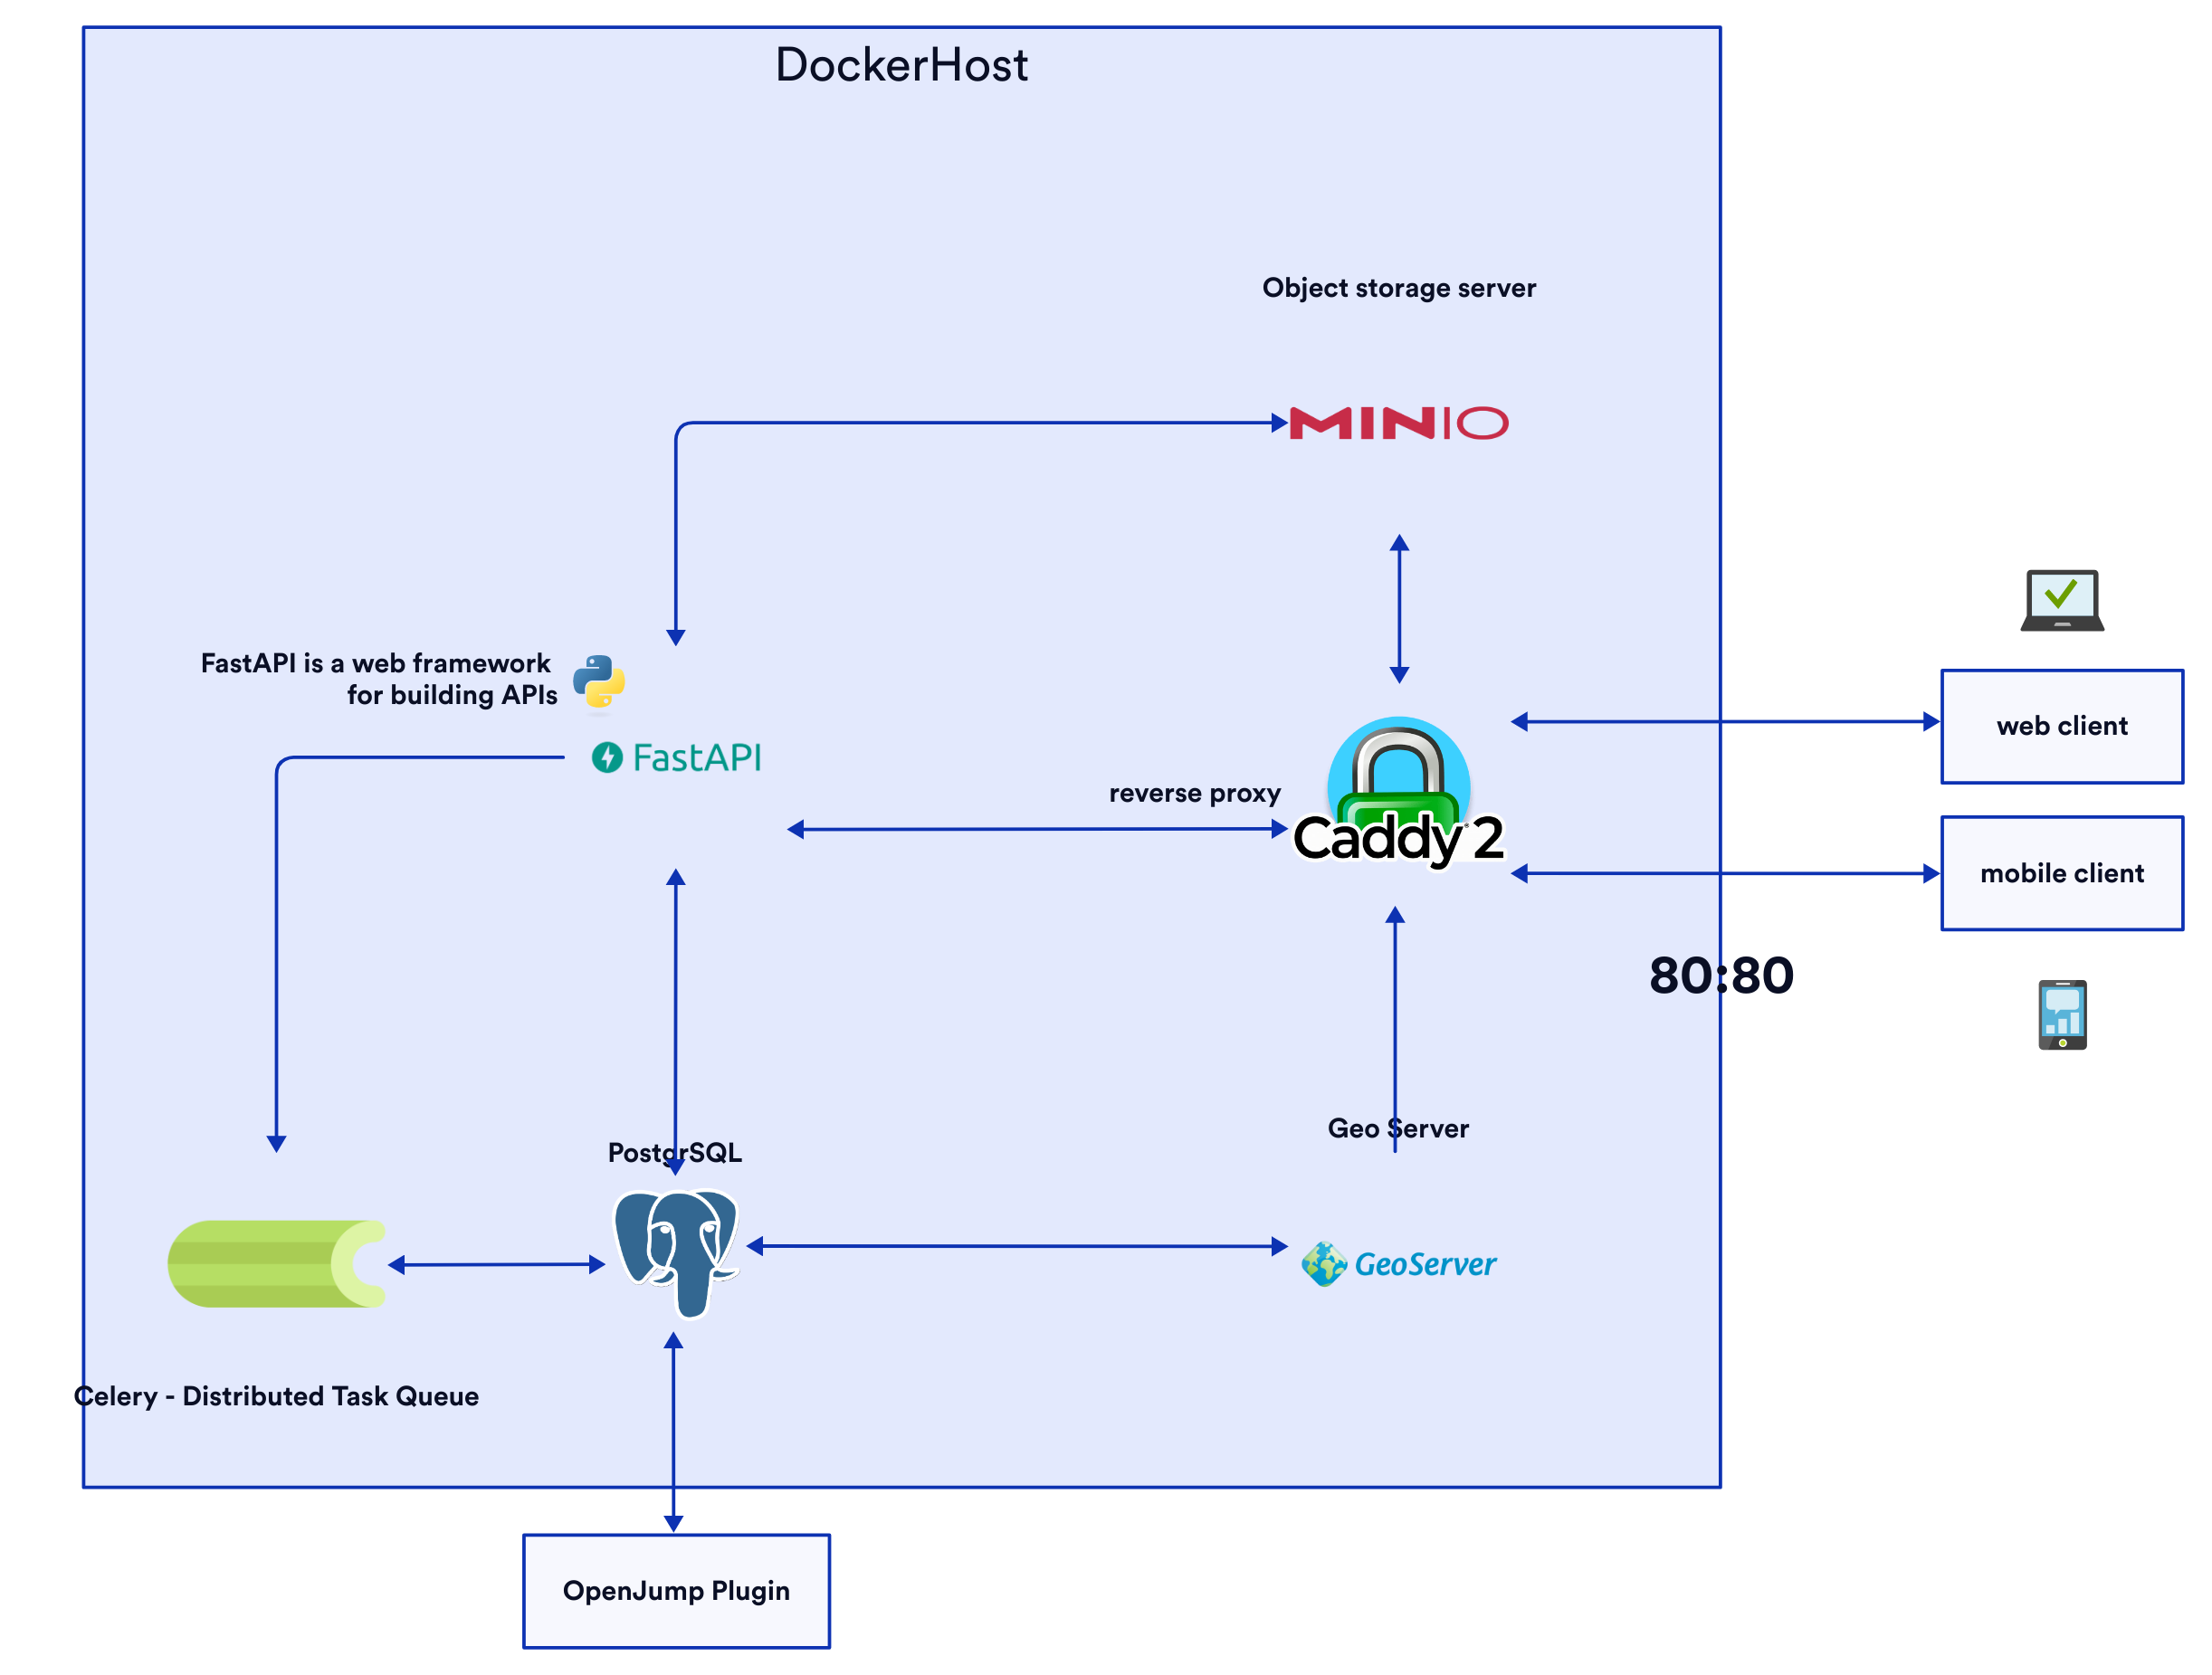
\includegraphics[width=\textwidth]{res/components_schema}
    \caption{components schema}
    \label{fig:components-schema}
\end{figure}

\section{Database}\label{sec:database}
\subsection{Initialize Database}\label{subsec:database-implementation}
Given data for Particelle data are provided in cadaster mode that relies on local reference points, we need to transform them into a global reference system.
To successfully carry out the conversion process, I meticulously followed a step-by-step procedure.
Initially, I identified the nearest \("\)punti fiduciali\("\) in proximity to the specific geographic area of interest, which in this case was in the vicinity of Fano.
These reference points held coordinates in both the Cassini Soldner and Gauss Braga coordinate reference systems (CRS).
By leveraging these paired coordinates, I constructed an Affine Transformation, a mathematical model capable of accurately converting coordinates from the Cassini Soldner system to the Gauss Boaga system.
This transformation was then methodically applied to the target cadastral data, facilitating a seamless and accurate conversion to the desired Gauss Boaga CRS.
The integration of these steps culminated in a robust and precise conversion process that was integral to the success of my research project.
The \("\)punti fiduciali\("\) dataset provided in OpenJump format was pivotal in enabling the smooth execution of this technique, reaffirming its value in overcoming the challenges associated with coordinate system conversions.

The Algorithm used to convert the coordinates is the following:
\begin{algorithm}[H]
    \caption{Calculate Transformation Matrix}
    \begin{algorithmic}[1]
        \REQUIRE $primary$, $secondary$
        \STATE $n \gets \text{shape of } primary[0]$
        \STATE $pad \gets \text{function that adds a column of ones to a given array}$
        \STATE $unpad \gets \text{function that removes the last column of a given array}$
        \STATE $X \gets pad(primary)$
        \STATE $Y \gets pad(secondary)$
        \STATE $A, res, rank, s \gets \text{result of solving least squares problem } X * A = Y$
        \STATE $transform \gets \text{function that applies the transformation matrix A to a given array}$
        \RETURN $transform$
    \end{algorithmic}\label{alg:algorithm}
\end{algorithm}

Now we're ready to create the database, we need to create a new database in PostgreSQL, and then we need to create the schema, the tables and the views.
We use shp2sql to import the shapefiles into the database.

\newpage

\subsection{Database Schema}\label{subsec:database-schema}
\begin{figure}[H]
    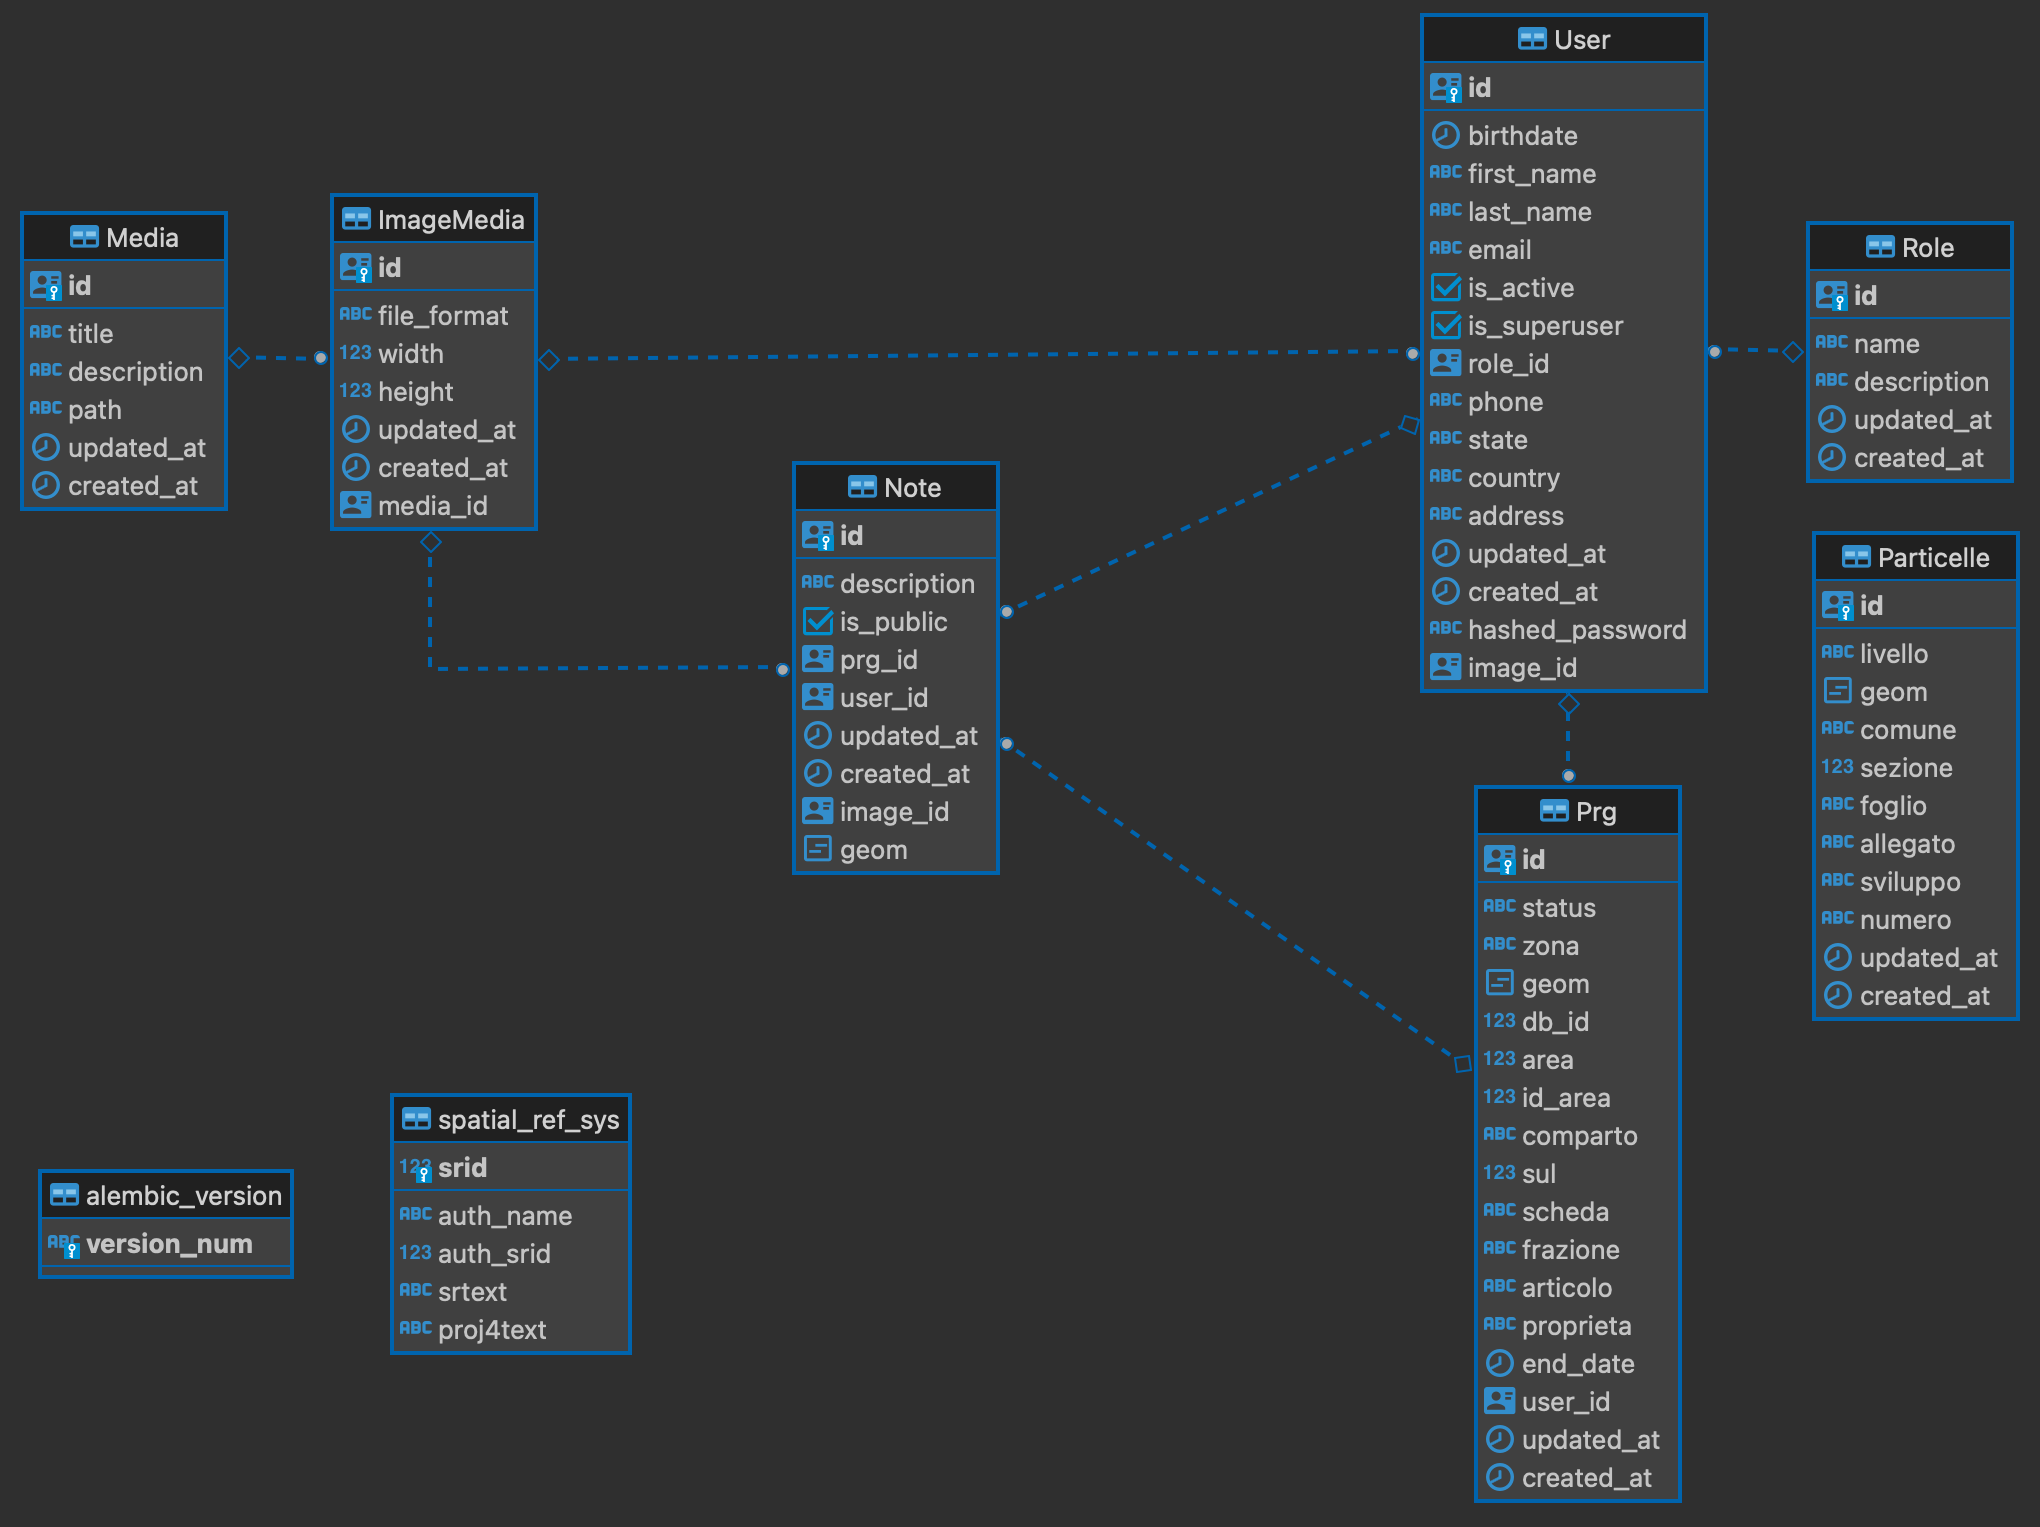
\includegraphics[width=\textwidth]{res/db_schema}
    \caption{db schema}
    \label{fig:dbschema}
\end{figure}

\subsection{Description of Entities and Relationships}\label{subsec:database-entity-relationship}
The relationships established between the tables in database schema play a crucial role in making the GIS project app work seamlessly. Let's delve deeper into how these relationships contribute to the functionality of the application:

\subsubsection{ImageMedia and Media Relationship}
The \texttt{ImageMedia} table contains information about image media files, while the \texttt{Media} table holds general media data. This relationship allows you to associate specific images with general media records. For example, you can link a particular image to a video or other media content. It enables the app to manage different types of media assets and efficiently retrieve associated images when needed.

\subsubsection{Note, ImageMedia, Prg, and User Relationships}
The \texttt{Note} table is at the core of the app, storing notes related to land usage. The relationships with \texttt{ImageMedia}, \texttt{Prg}, and \texttt{User} are fundamental for organizing and contextualizing the notes. The connection with \texttt{ImageMedia} allows users to associate images with their notes, enhancing the visual representation of the content. The link to \texttt{Prg} helps tie notes to specific land usage plans, enabling users to provide location-specific information and feedback. The relationship with \texttt{User} ensures that each note is attributed to a specific user, facilitating accountability and user-specific access to notes.

\subsubsection{Prg and User Relationship}
The \texttt{Prg} table represents urban recovery and redevelopment plans. The relationship with \texttt{User} is essential for assigning responsibility for the plans to specific users. This connection allows administrators and designated users to manage and update the details of the plans they are responsible for.

\subsubsection{User and ImageMedia, Role Relationships}
The \texttt{User} table represents app users, including administrators and regular users. The relationship with \texttt{ImageMedia} allows users to have profile images associated with their accounts. This enhances the user experience by enabling users to personalize their profiles and providing a visual identification. The connection with \texttt{Role} defines user roles and permissions, making it possible to differentiate between administrators and regular users. Role-based access control ensures that only authorized users can perform certain actions, enhancing security and data integrity.

\subsubsection{Overall Functionality}
These relationships collectively enable the GIS project app to provide the following functionalities:

\begin{itemize}
    \item User Authentication and Authorization
    \item Land Usage Notes and Planning
    \item Media Management
    \item User Profiles
    \item Responsibility Assignment
\end{itemize}

In summary, the well-defined relationships in the database schema are the backbone of the GIS project app, enabling seamless interactions between different entities, data organization, user authentication, access control, and efficient management of land usage data for the city.


\section{Functional Aspects of the System}\label{sec:functional-aspects-of-the-system}
\subsection{WebGIS Application}\label{subsec:fa-webgis-application}
Our web application is mainly composed of 5 parts:
\begin{enumerate}
    \item \textbf{Displaying Parts and Variants}: To display public data to all users and provide technicians with access to manage them.
    \item \textbf{Notes and Comments}: Users have the ability to write notes and comments for various variants or create a polygon to add notes to. Additionally, users can view all public notes.
    \item \textbf{Creating Variants}: Technicians can draw new areas and incorporate them as variants. These variants remain inactive and are not visible to the public.
    \item \textbf{Managing Variants}: Modifying the status of variants and making them visible to all users.
    \item \textbf{Search and Print}: Searching for parts and printing the associated area with its details.
\end{enumerate}

Main Page of the application
\begin{figure}[H]
    \centering
    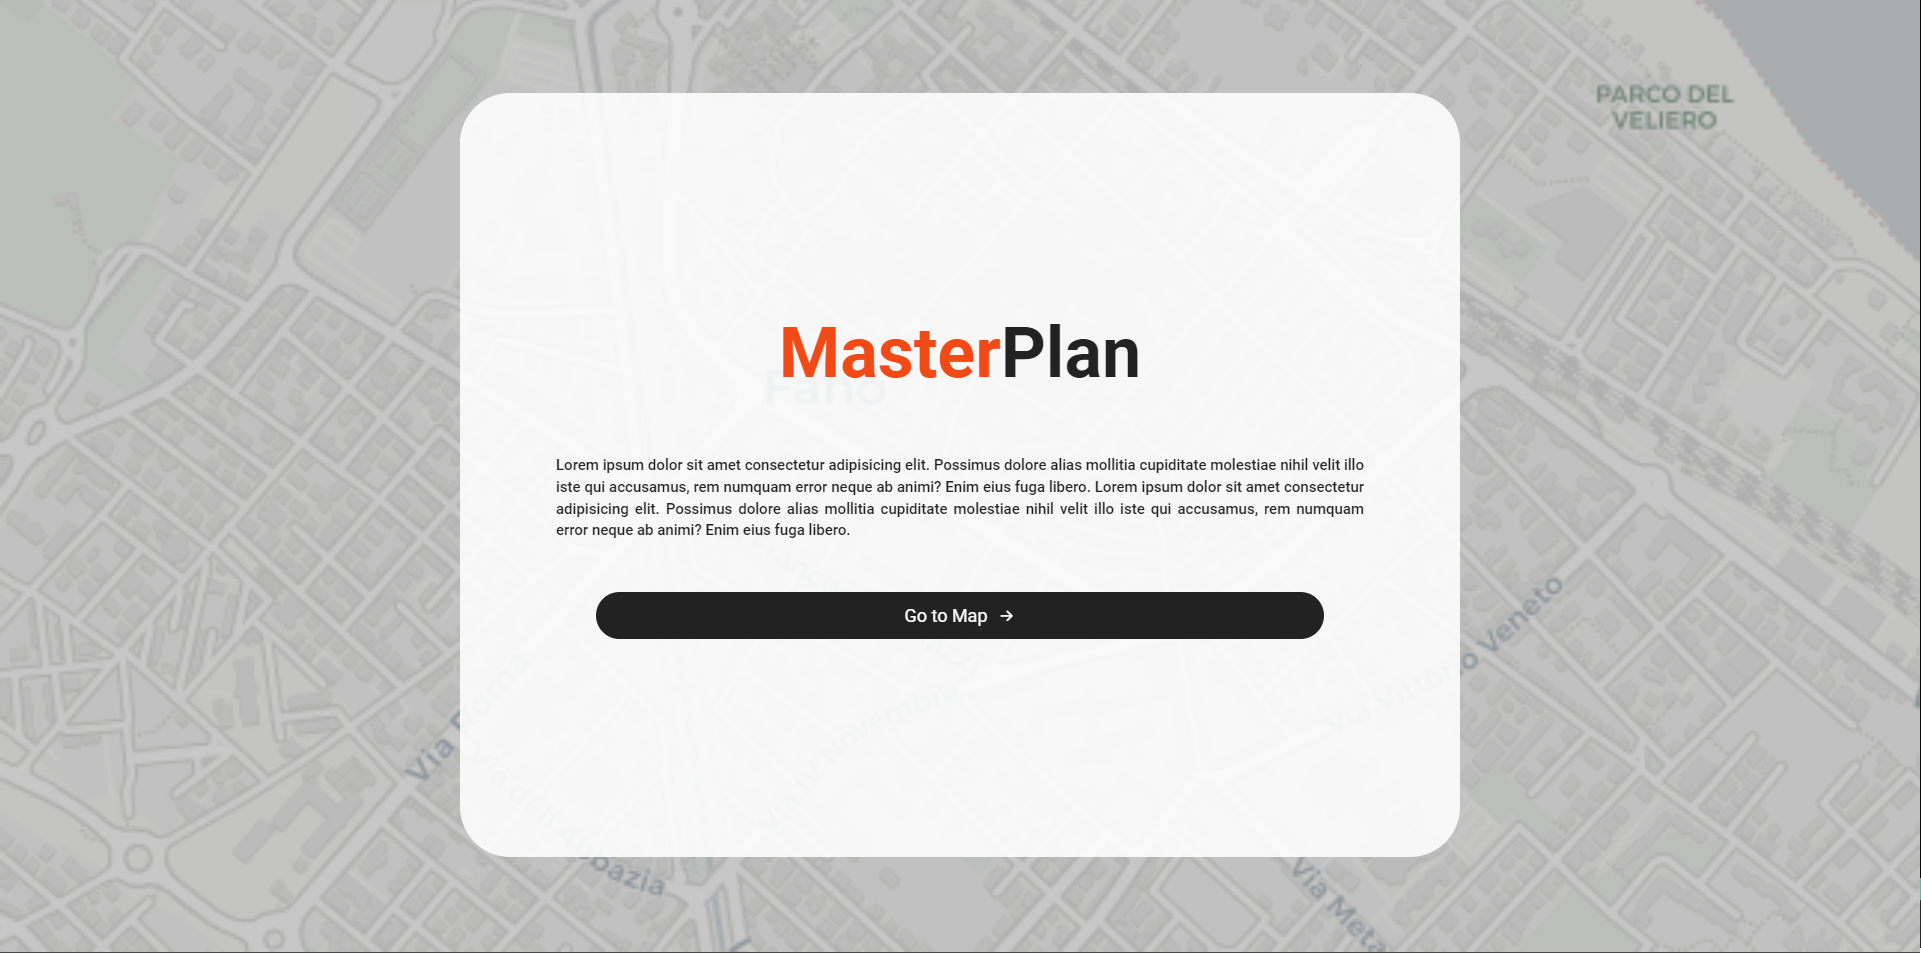
\includegraphics[width=0.9\textwidth]{res/web/1-maste-plan intro}
    \caption{The first page presents temporary data to help users quickly grasp the app's context}
    \label{fig:web-main}
\end{figure}

Login and Registration procedure for users (esp: for technicians)
\begin{figure}[H]
    \centering
    \begin{minipage}{0.48\textwidth}
        \centering
        
\includegraphics[width=\textwidth]{res/web/2-register}
        \caption{Login Page}
        \label{fig:web-login}
    \end{minipage}
    \hfill
    \begin{minipage}{0.48\textwidth}
        \centering
        
\includegraphics[width=\textwidth]{res/web/3-register}
        \caption{Registration page}
        \label{fig:web-register}
    \end{minipage}
\end{figure}


Explore the interface where parts and their variations are showcased, accessible to both the public and technicians:
\begin{figure}[H]
    \centering
    \begin{minipage}{0.48\textwidth}
        \centering
        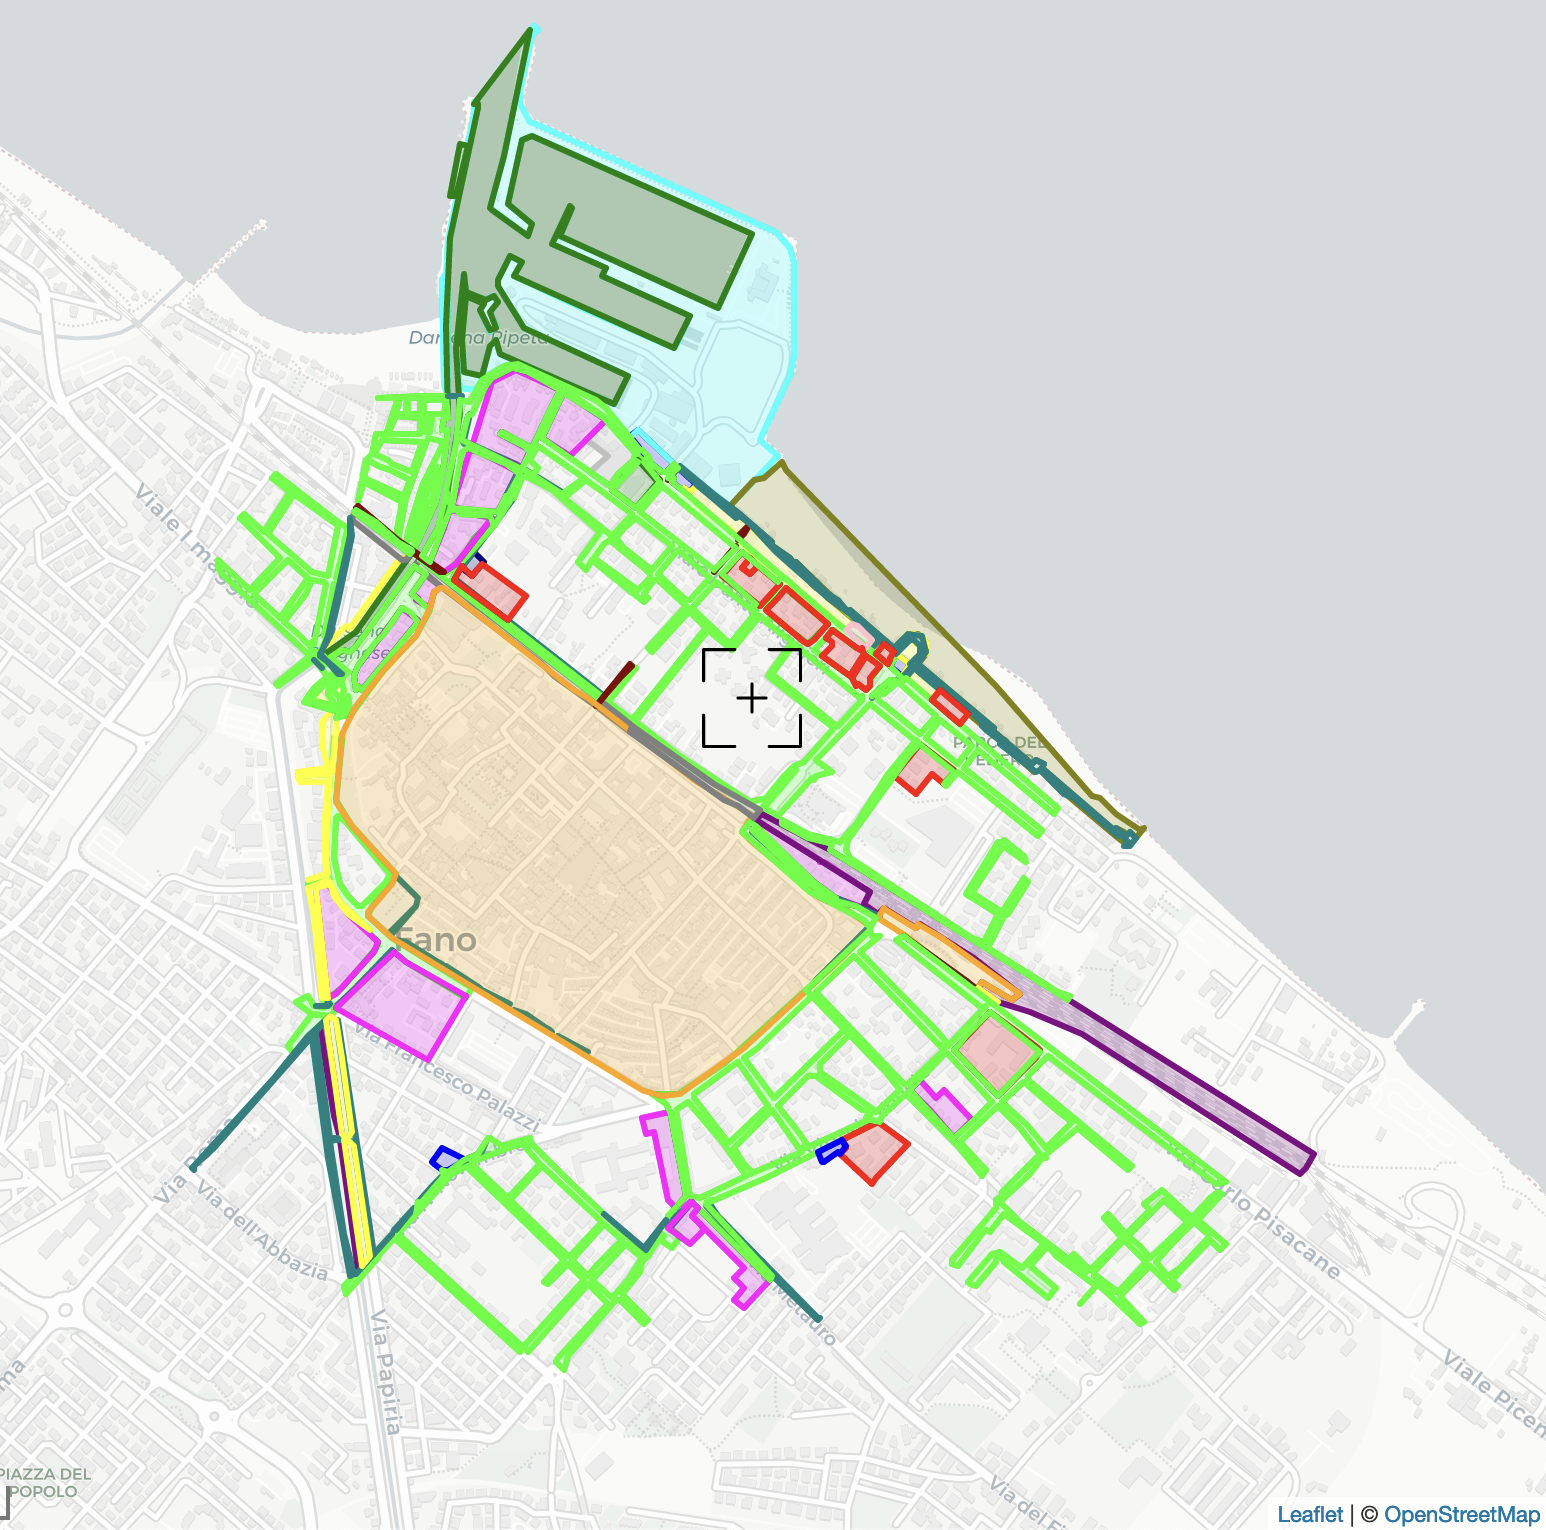
\includegraphics[width=\textwidth]{res/web/map-data}
        \caption{Variants}
        \label{fig:web-map-data}
    \end{minipage}
    \hfill
    \begin{minipage}{0.48\textwidth}
        \centering
        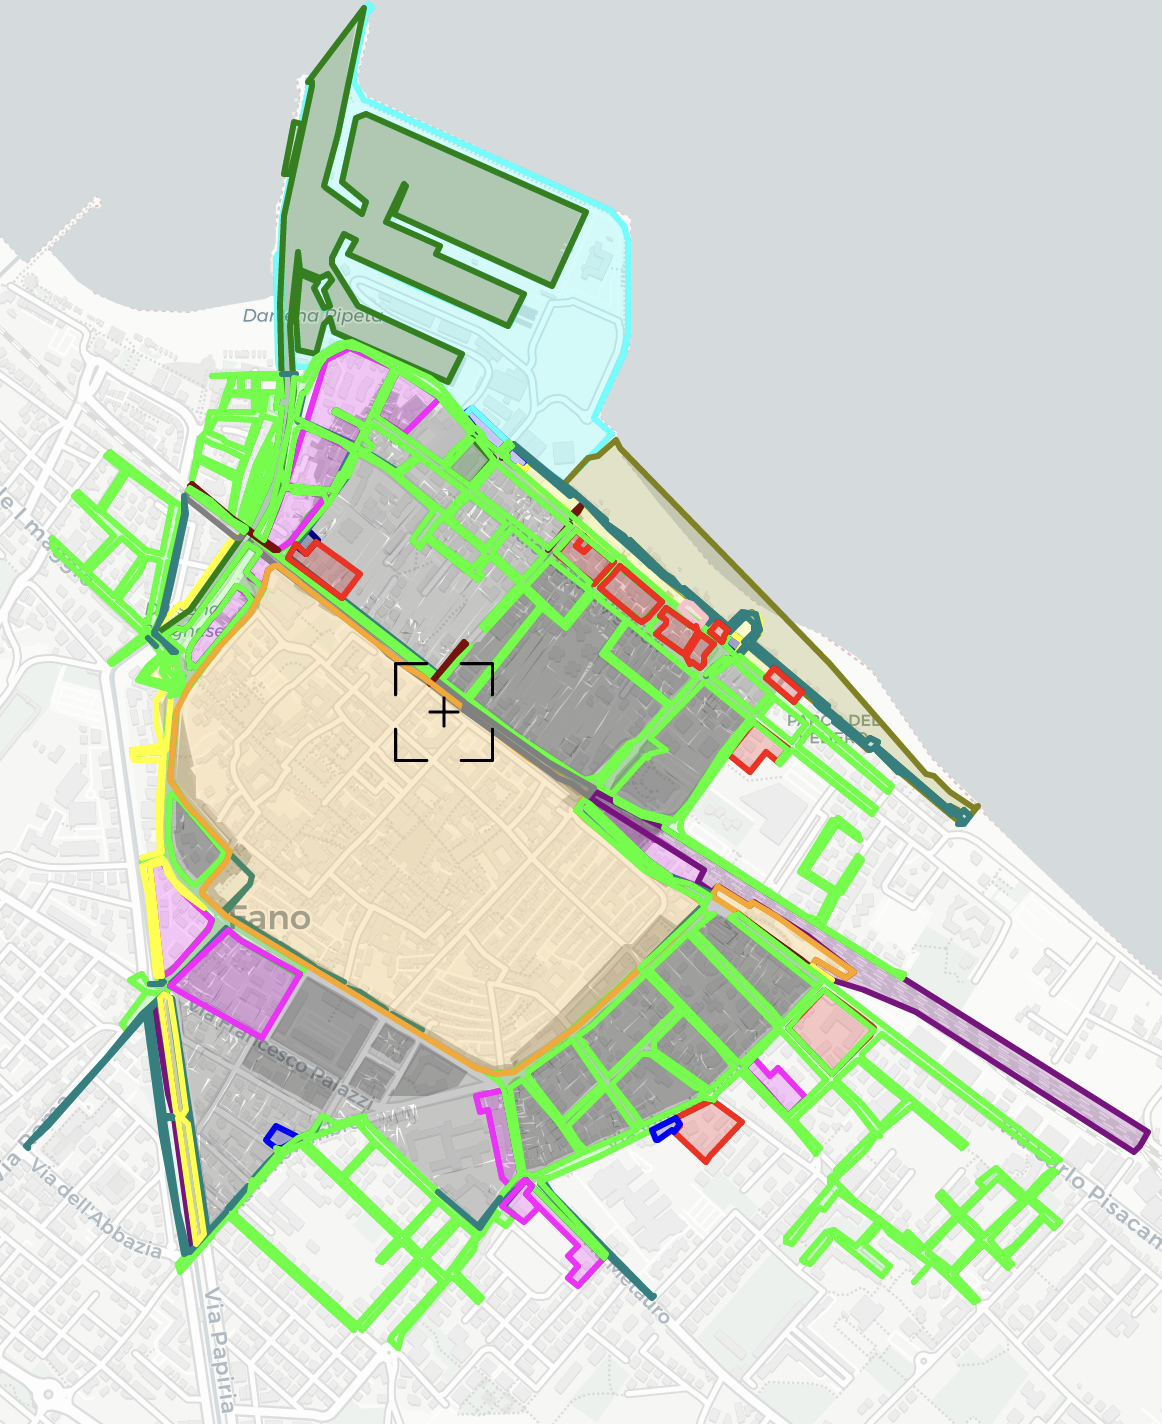
\includegraphics[width=\textwidth]{res/web/both-map-data}
        \caption{Parcels + Variants}
        \label{fig:web-map-all-data}
    \end{minipage}
\end{figure}


Discover how users interact with the system by writing notes and comments for different variants or creating polygons for additional context.
Observe the display of public notes.
\begin{figure}[H]
    \centering
    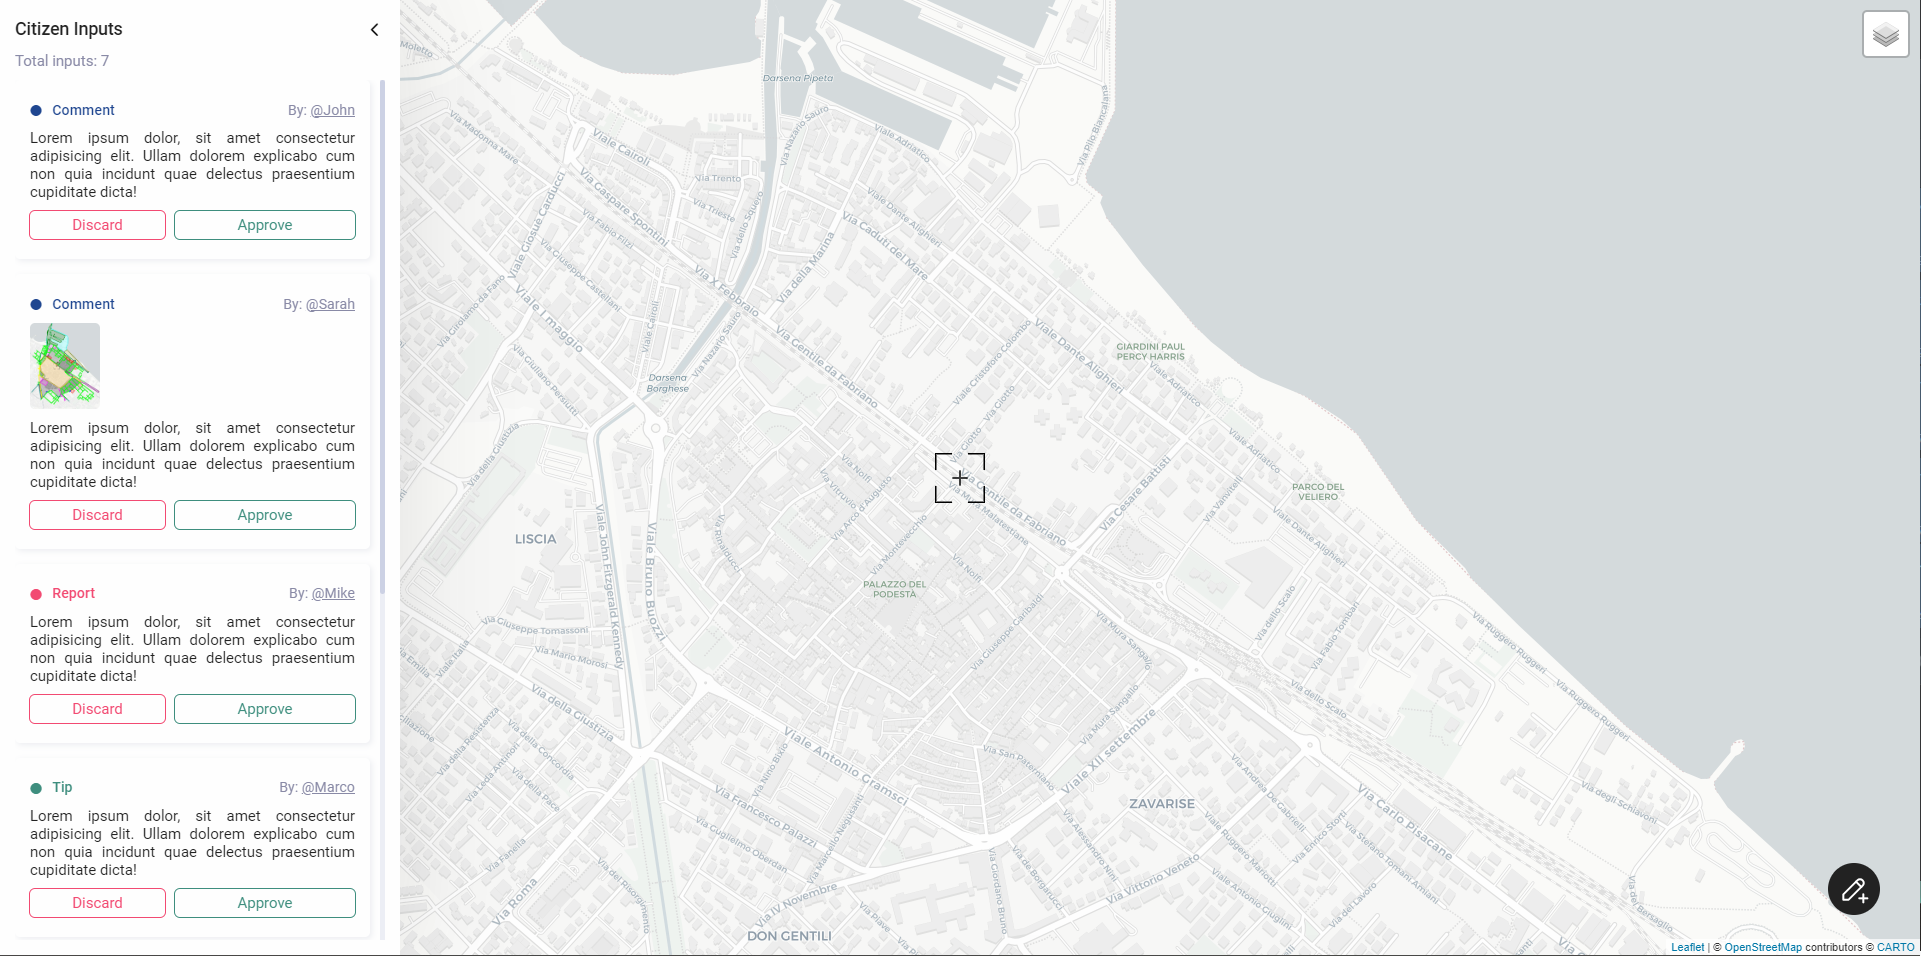
\includegraphics[width=0.9\textwidth]{res/web/notes-main}
    \caption{User interaction with notes, comments, and polygons, with public notes displayed.}
    \label{fig:web-notes}
\end{figure}

\begin{figure}[H]
    \centering
    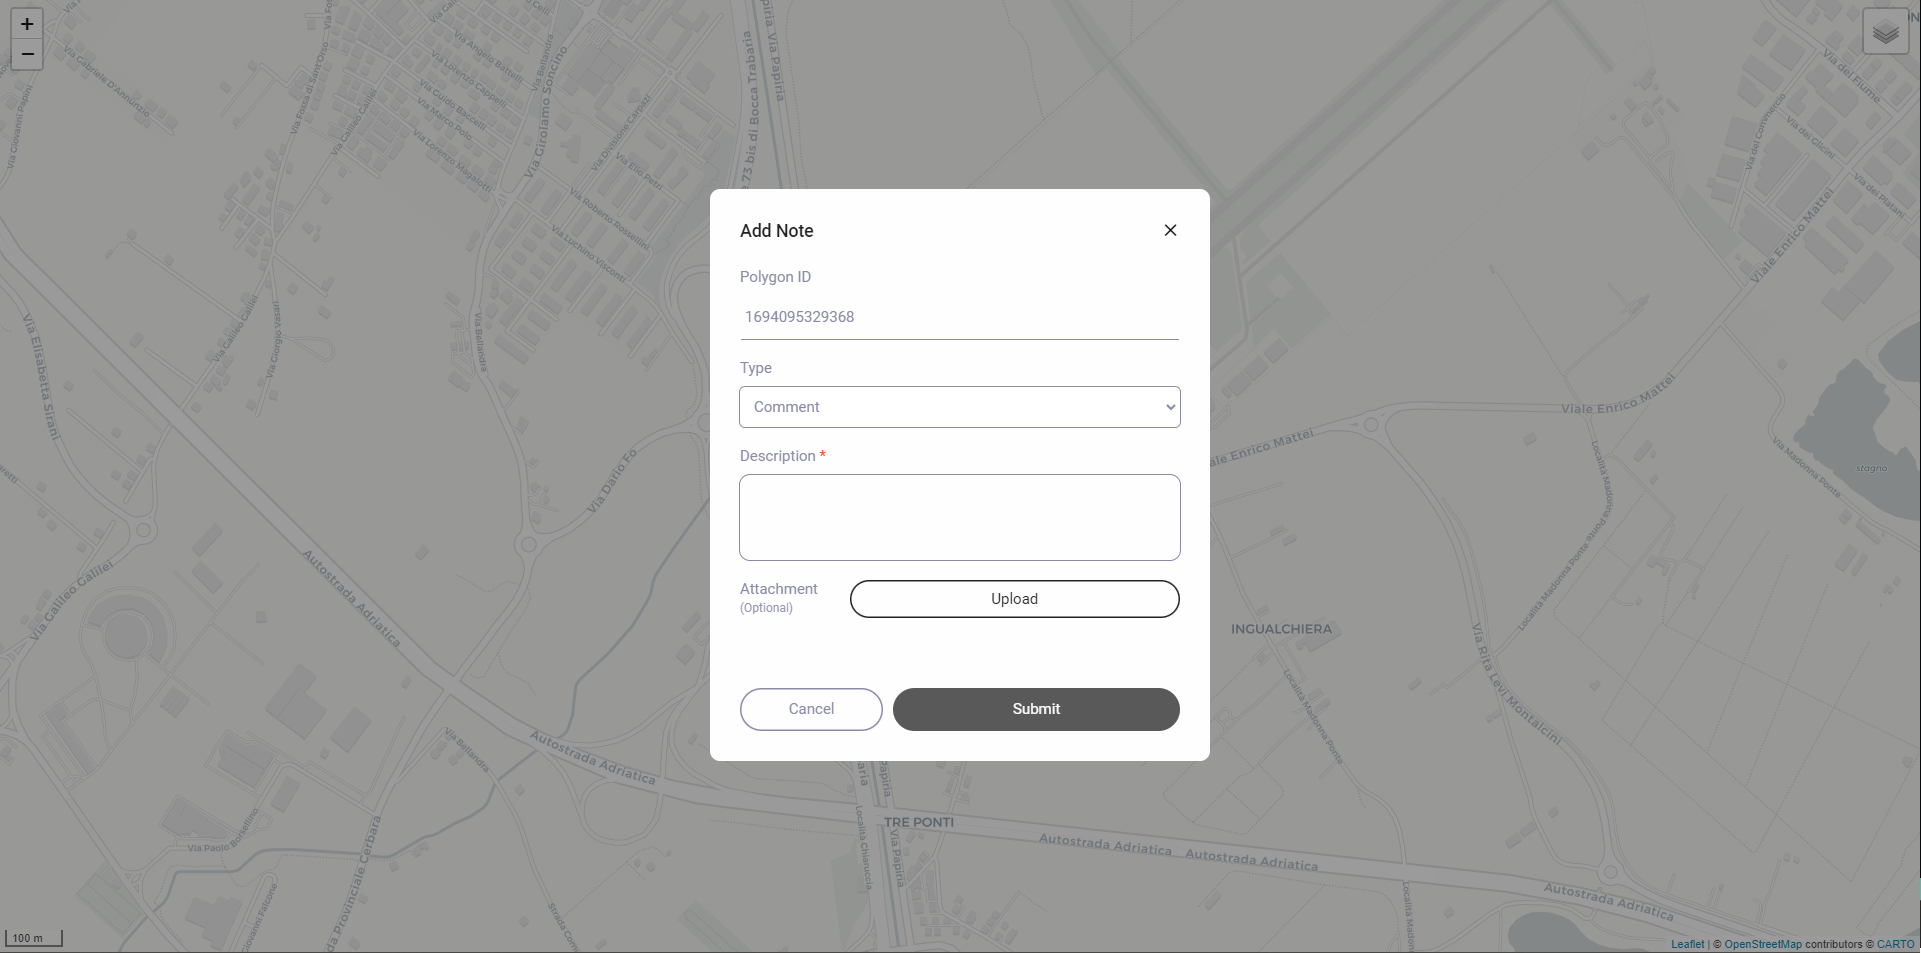
\includegraphics[width=0.9\textwidth]{res/web/add-note}
    \caption{Adding Notes}
    \label{fig:web-add-note}
\end{figure}

Witness technicians drawing and incorporating new areas as variants within the system.
These additions are initially hidden from public view.
+ Observe the process of modifying the status of variants and making them visible to all users for effective management.
\begin{figure}[H]
    \centering
    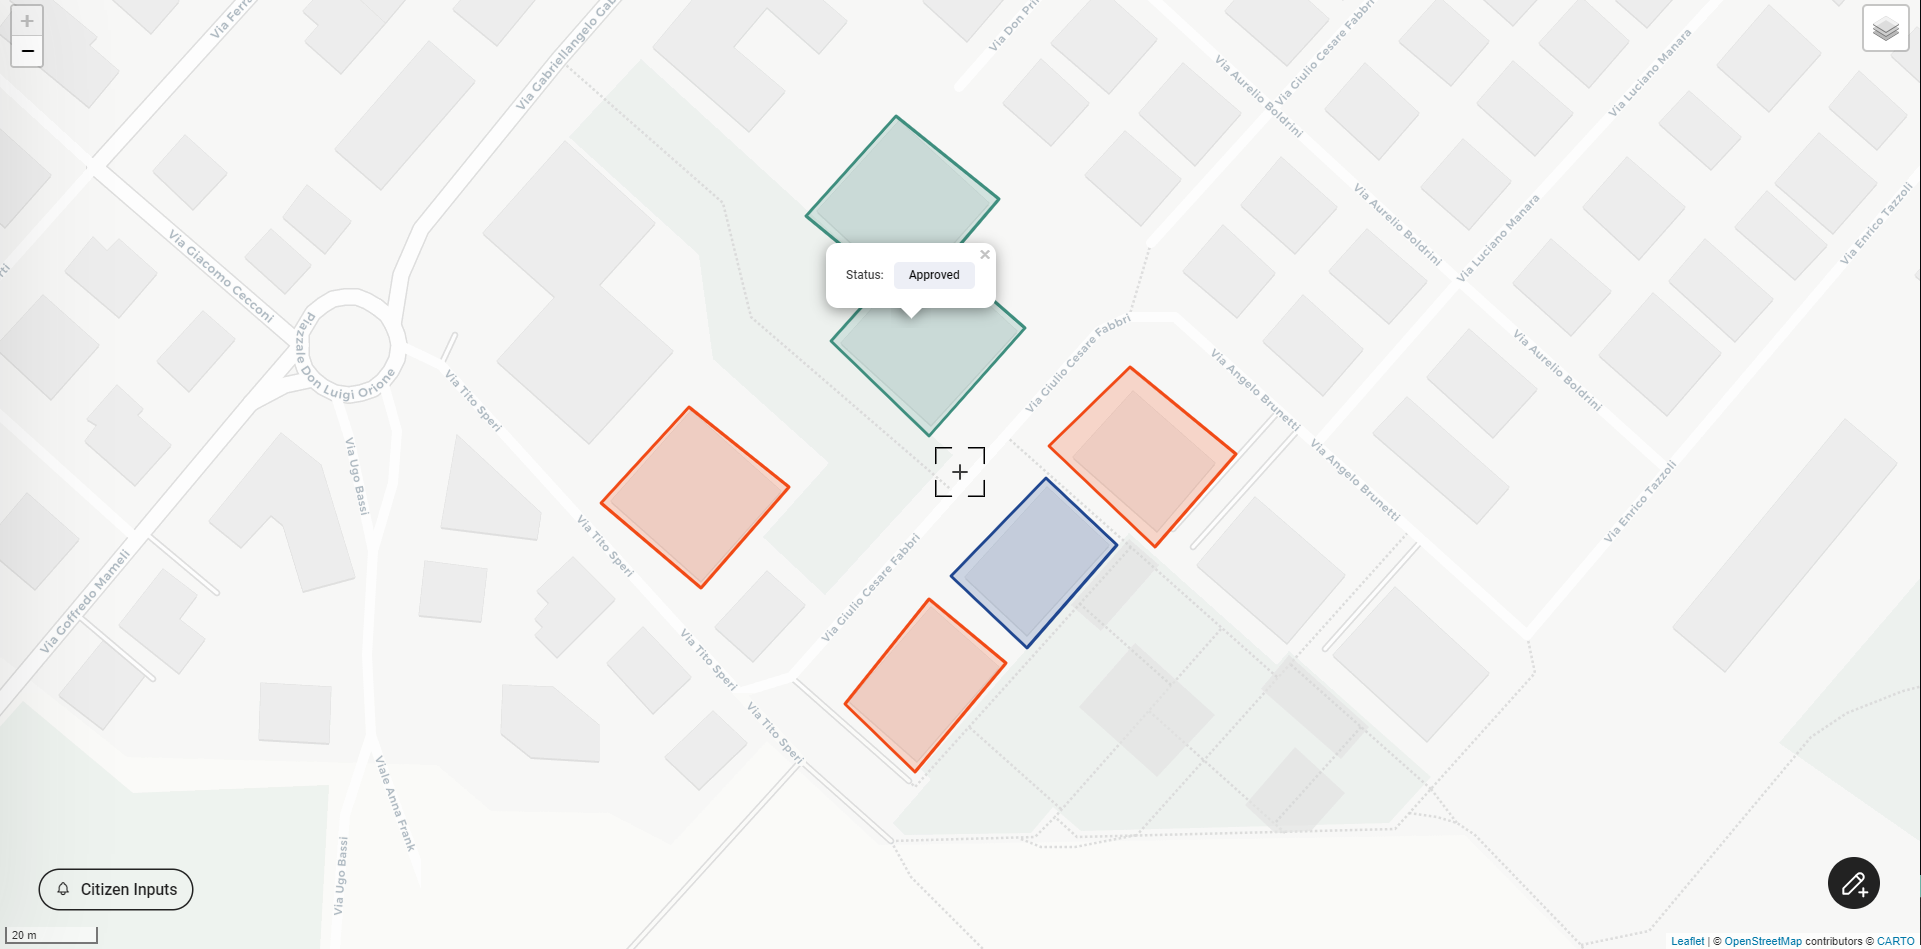
\includegraphics[width=0.9\textwidth]{res/web/4-draw polygons}
    \caption{Administering variant.}
    \label{fig:web-create-var}
\end{figure}

%Observe the process of modifying the status of variants and making them visible to all users for effective management.
%\begin{figure}[H]
%    \centering
%    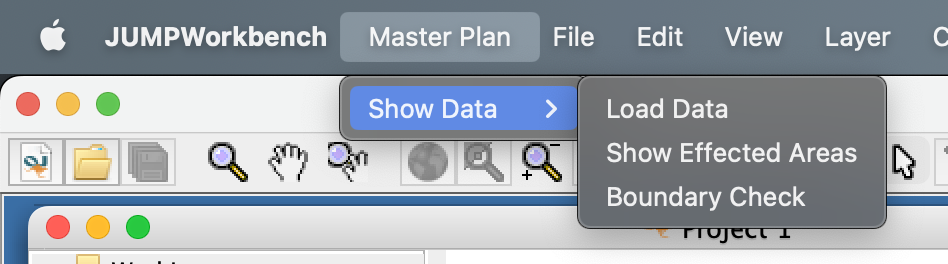
\includegraphics[width=0.8\textwidth]{res/plugin/01-menu}
%    \caption{Administering variant status and making them visible to all users.}
%    \label{fig:web-edit-var}
%\end{figure}

%Explore the functionalities of searching for specific parts and printing detailed information along with their associated areas for convenient reference.
%\begin{figure}[H]
%    \centering
%    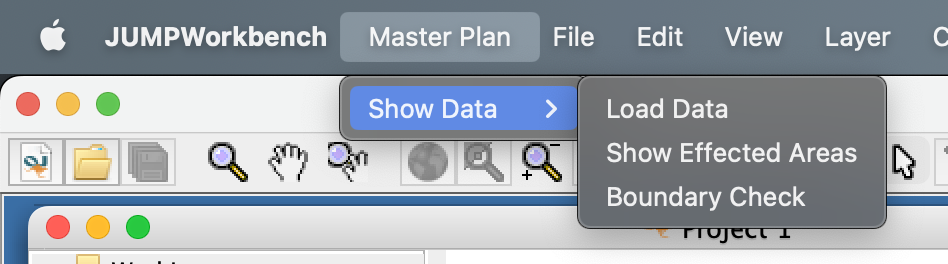
\includegraphics[width=0.8\textwidth]{res/plugin/01-menu}
%    \caption{Utilizing search functionality and printing part details with associated areas.}
%    \label{fig:web-search}
%\end{figure}


Mobile Compatible version
\begin{figure}[H]
    \centering
    \begin{minipage}{0.24\textwidth}
        \centering
        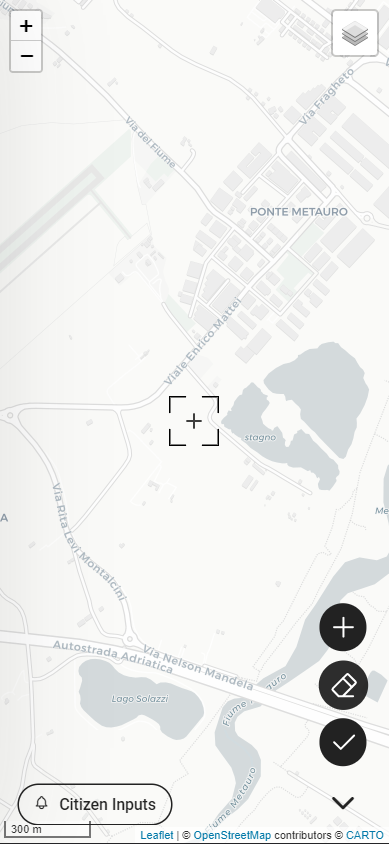
\includegraphics[width=\textwidth]{res/web/mobile-app}
    \end{minipage}
    \hfill
    \begin{minipage}{0.24\textwidth}
        \centering
        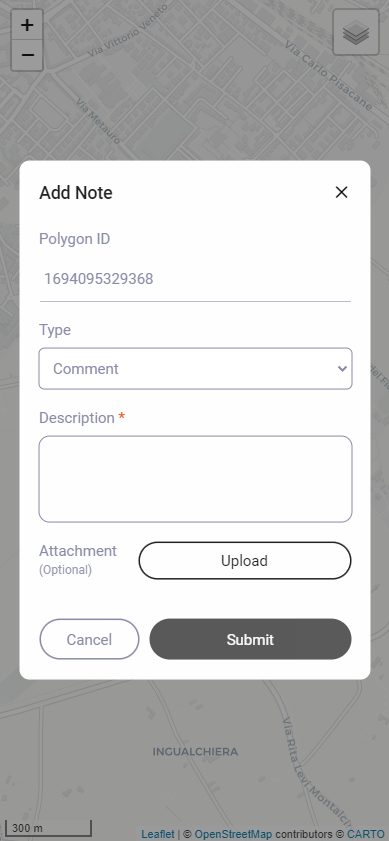
\includegraphics[width=\textwidth]{res/web/mobile-add-note}
    \end{minipage}
    \hfill
    \begin{minipage}{0.24\textwidth}
        \centering
        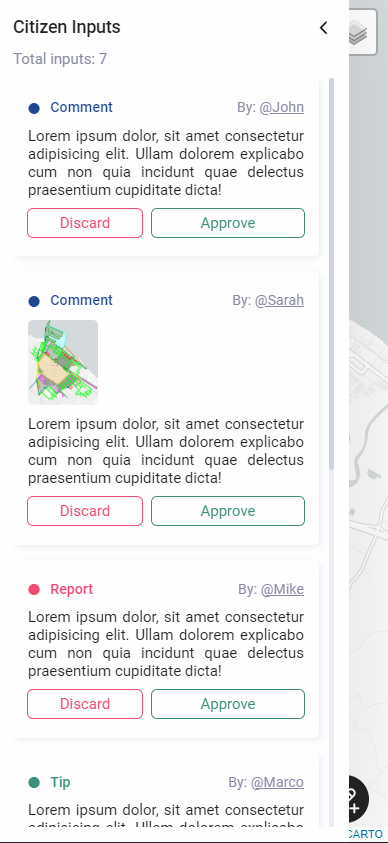
\includegraphics[width=\textwidth]{res/web/mobile-see-notes}
    \end{minipage}
    \hfill
    \begin{minipage}{0.24\textwidth}
        \centering
        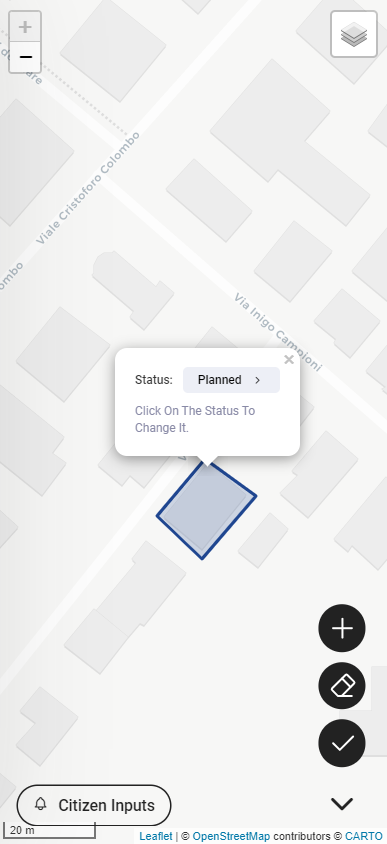
\includegraphics[width=\textwidth]{res/web/mobile-change-status}
    \end{minipage}
    \caption{Responsive application}\label{fig:mobile-compatiable}
\end{figure}

\subsection{OpenJUMP plugin}\label{subsec:fa-openjump-plugin}
Our plugin is composed of 3 main parts:
\begin{enumerate}
    \item \textbf{Load data from the database}: this part is responsible for loading the data from the database, the data are loaded in the form of layers, and the layers are loaded in the form of features.
    \item \textbf{Show Effect Areas}: this part is responsible for showing the effect areas of the variants, the effect areas are the areas that are affected by the variant.
    \item \textbf{Boundary}: this part is responsible for showing the boundary of the effect areas, checking if the boundary is correct, and showing the parcels that are excluded or partially included.
\end{enumerate}

For each part, we have a menu item, and each menu item has a button that is responsible for activating the part.
\begin{figure}[H]
    \centering
    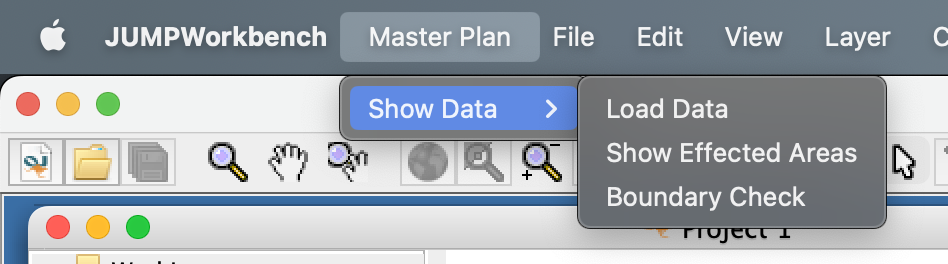
\includegraphics[width=0.8\textwidth]{res/plugin/01-menu}
    \caption{Menu of the plugin}
    \label{fig:pl-menu}
\end{figure}

After loading the data from the database, we can see the layers in the layer panel, and we can see the features in the map panel.
\begin{figure}[H]
    \centering
    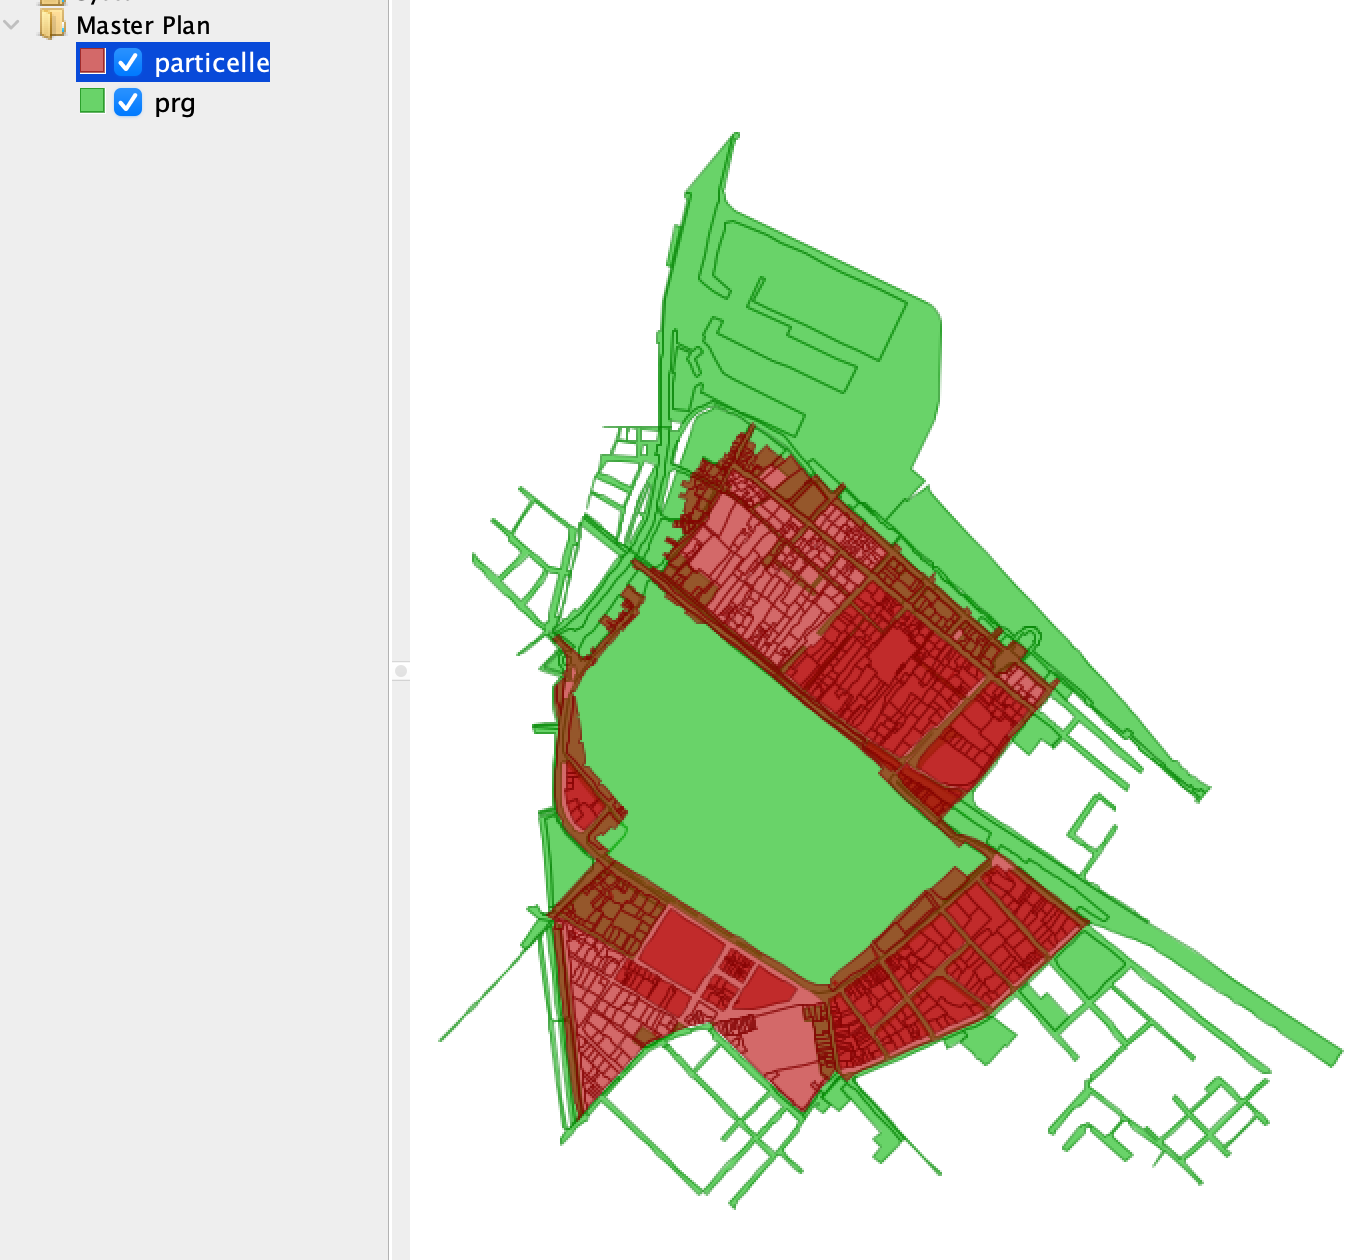
\includegraphics[width=0.8\textwidth]{res/plugin/02-load-data}
    \caption{Load data from the database}
    \label{fig:pl-load-data}
\end{figure}

For seeing the effect areas, we need to choose a variant, and then we can see the effect areas of the variant.
We choose the variant from the drop down menu, these item id are the id of the variants in the database.
\begin{figure}[H]
    \centering
    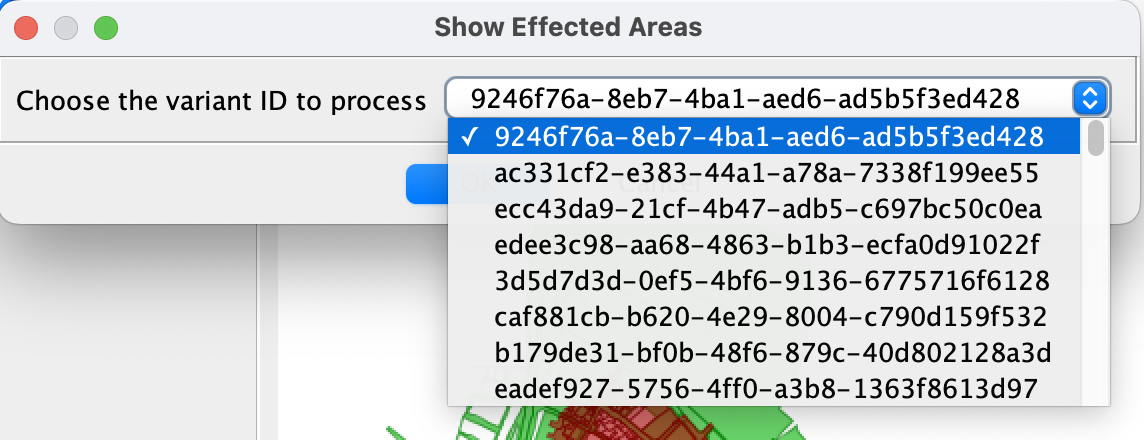
\includegraphics[width=0.8\textwidth]{res/plugin/03-show-areas}
    \caption{Show fffect areas - Choose a variant}
    \label{fig:pl-show-areas}
\end{figure}

After choosing the variant, we can see the effect areas of the variant.
For simplicity, we show them under the variant layer and the layer name is \texttt{variant\-variant\_id}.
\begin{figure}[H]
    \centering
    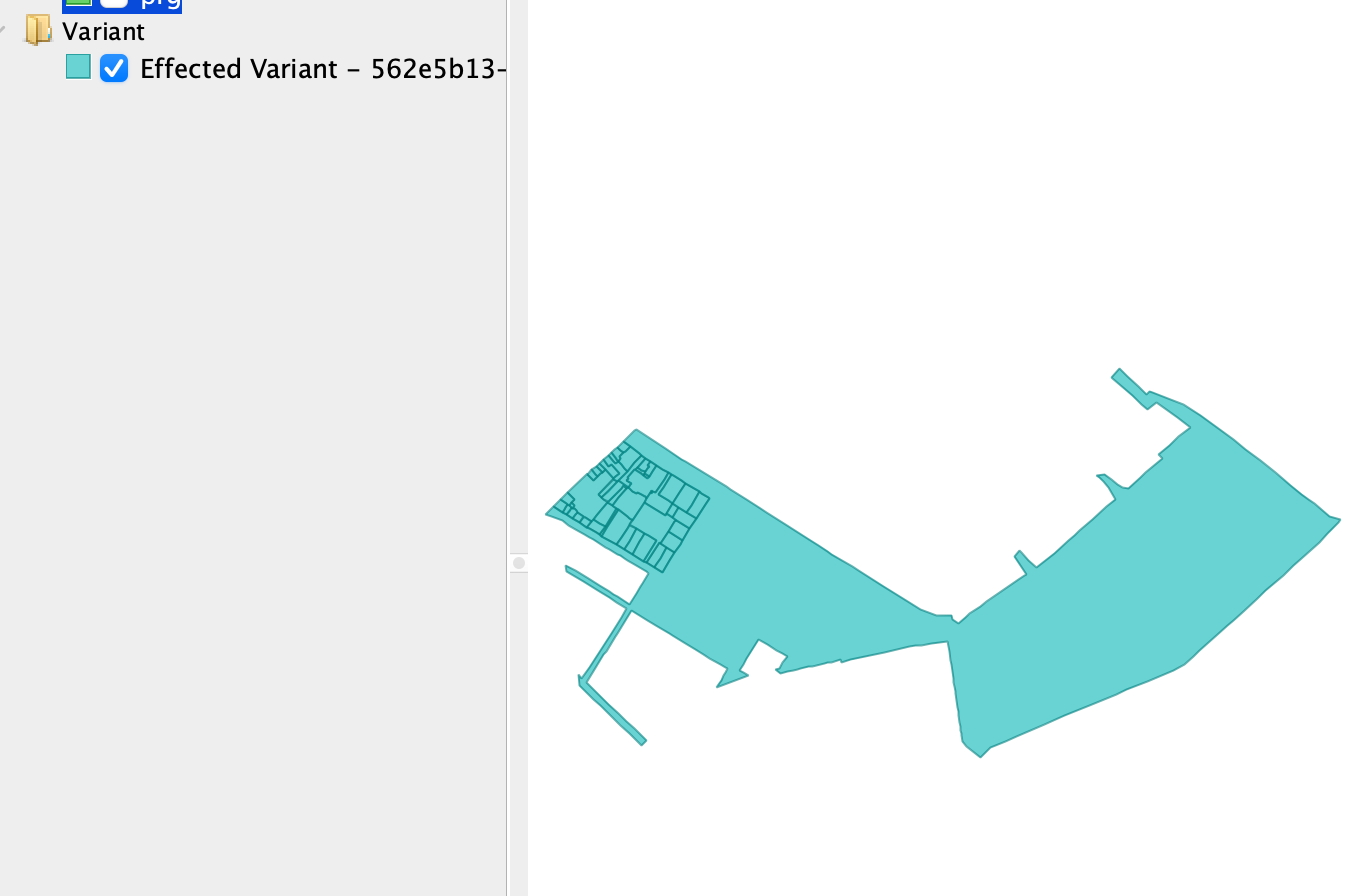
\includegraphics[width=0.8\textwidth]{res/plugin/04-show-areas}
    \caption{Show Effect Areas}
    \label{fig:pl-show-areas-2}
\end{figure}

In boundary part, we help the user to check if the boundary of the effect areas is correct or not.
We show the parcels that are excluded or partially included in the effect areas.
\begin{figure}[H]
    \centering
    \begin{minipage}{0.48\textwidth}
        \centering
        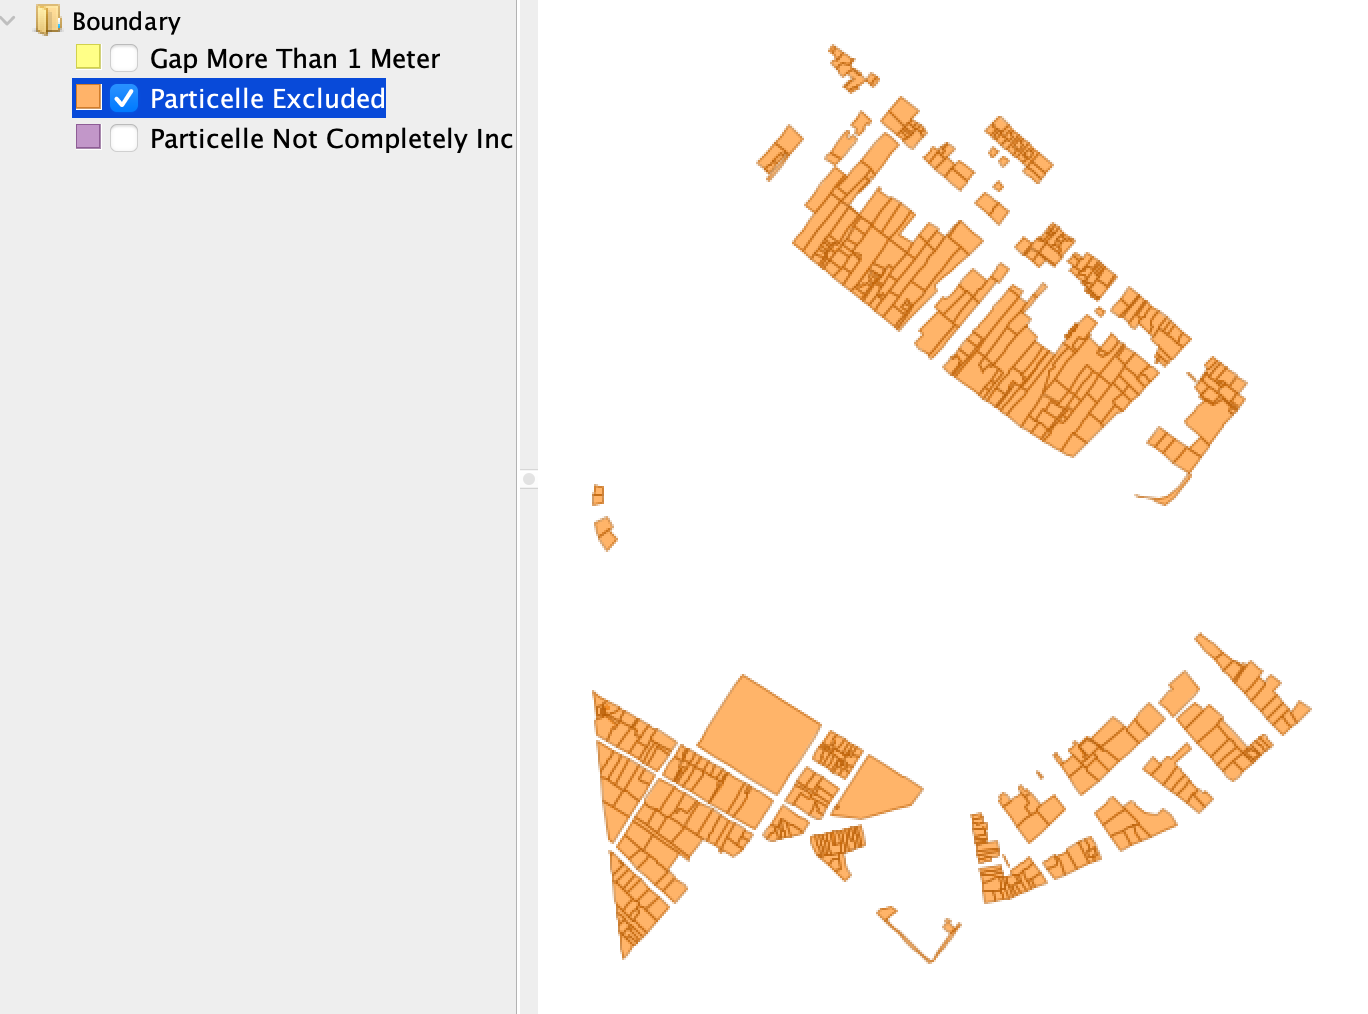
\includegraphics[width=\textwidth]{res/plugin/05-boundary}
        \caption{Parcels excluded}
        \label{fig:pl-boundary}
    \end{minipage}
    \hfill
    \begin{minipage}{0.48\textwidth}
        \centering
        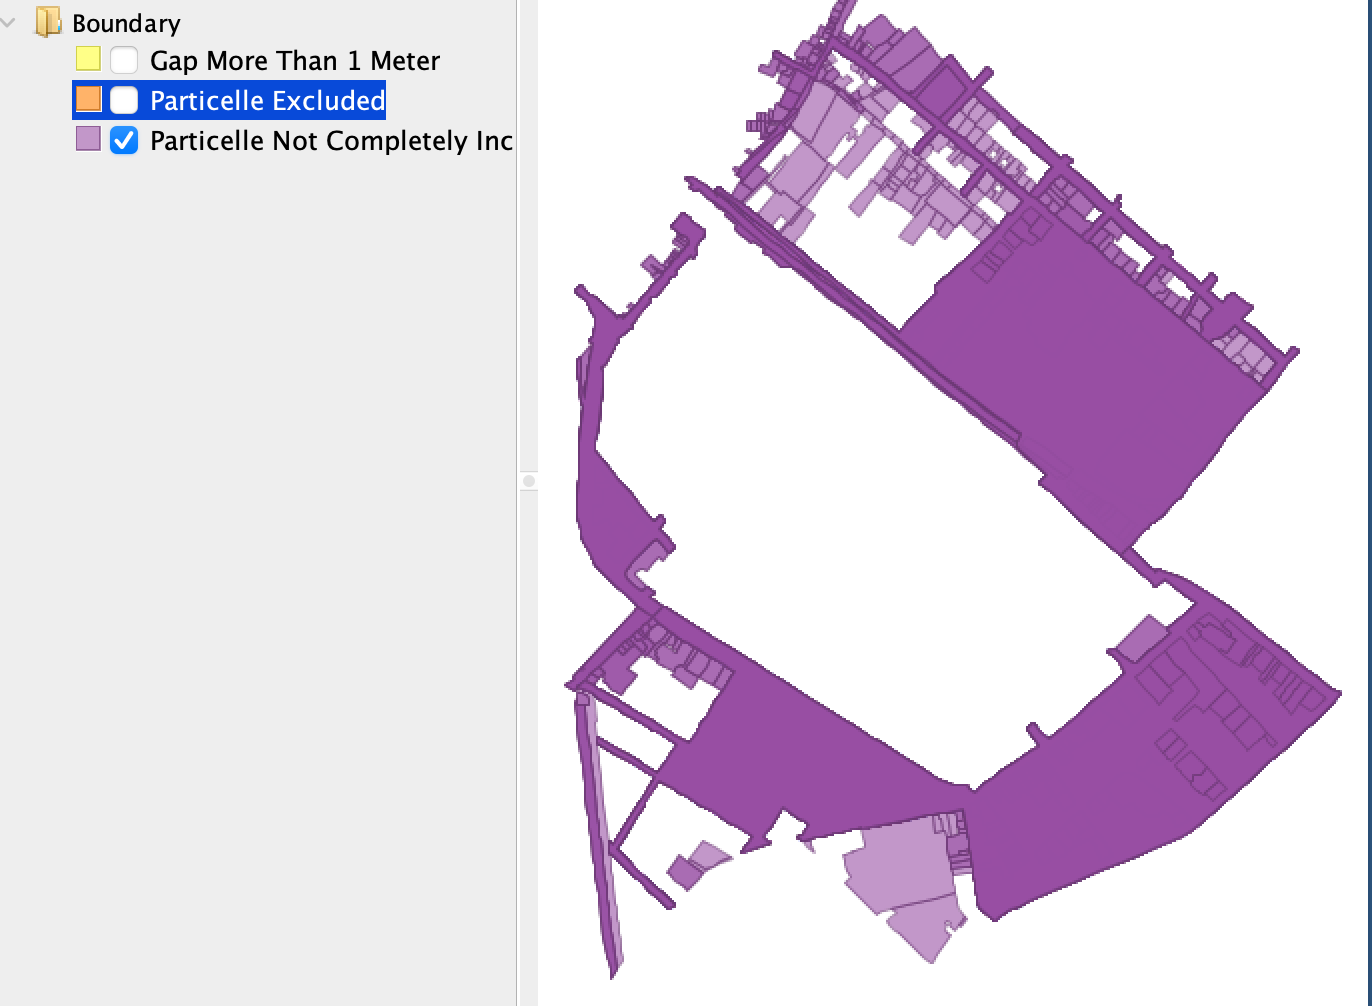
\includegraphics[width=\textwidth]{res/plugin/06-boundary.png}
        \caption{Parcels partially included}
        \label{fig:pl-boundary-2}
    \end{minipage}
\end{figure}

And we also show the gap between parcels and variant boundary if the gap is in threshold of 1 meter.
\begin{figure}[H]
    \centering
    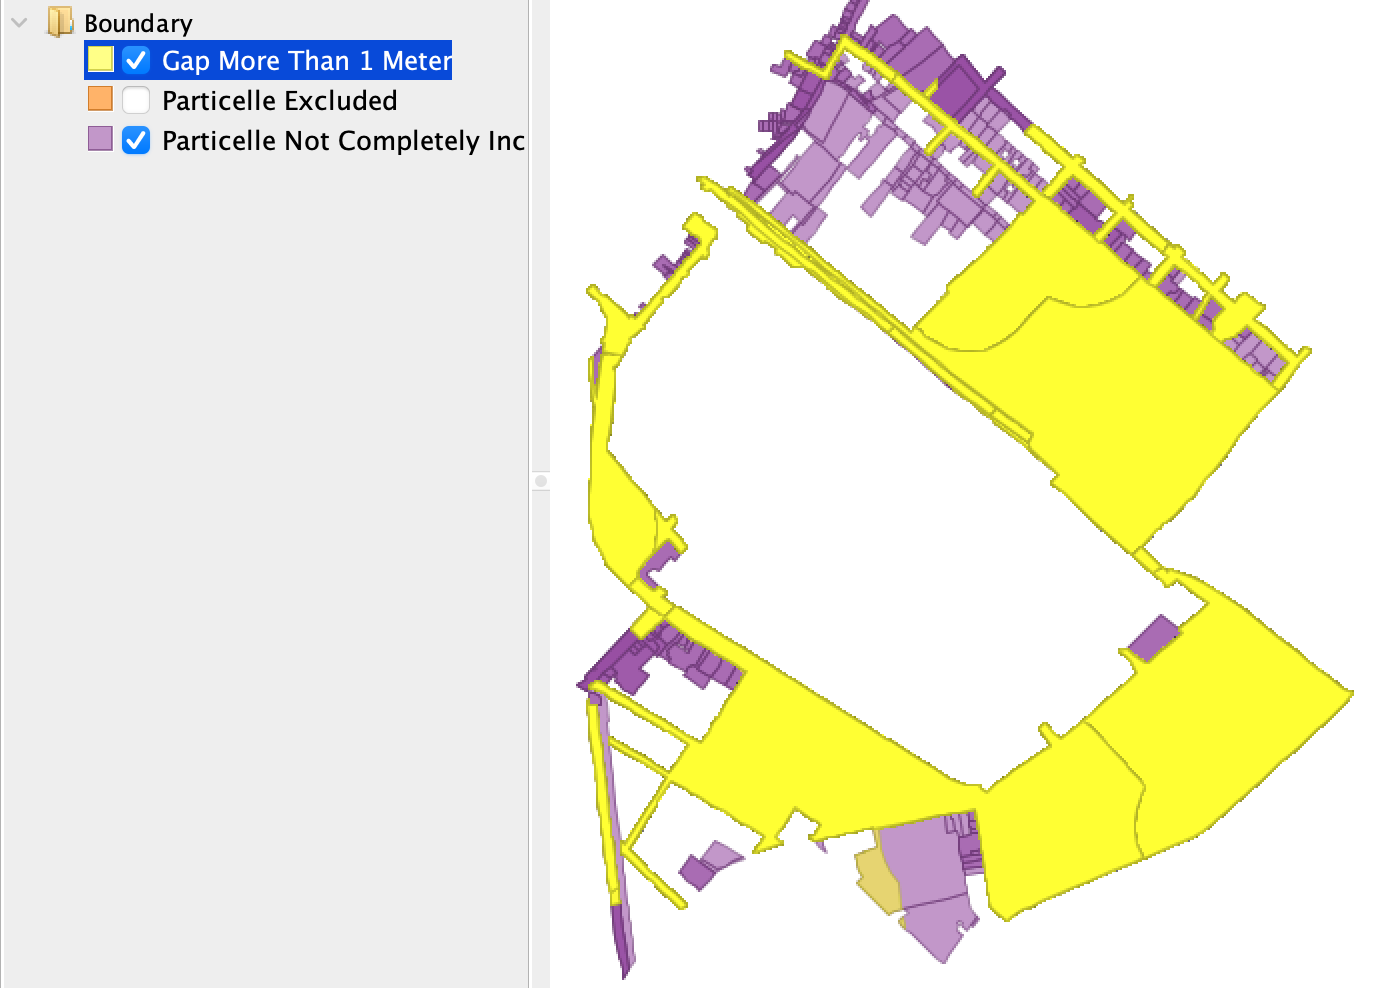
\includegraphics[width=0.8\textwidth]{res/plugin/07-boundary.png}
    \caption{Gap between parcels that partially included}
    \label{fig:pl-boundary-3}
\end{figure}